% Given a symptom rather than a known fault, which tool to reach for.
%
% The four faults in this project are labelled, so the matrix figure can
% be read off them. This one starts from the situation you are actually
% in, where nobody has told you which fault it is, and the first question
% is not about the bug: it is whether the board is still running.
\documentclass[tikz, border=4pt]{standalone}
% Shared styles for the Project 9 figures.
%
% Every figure in this directory is standalone: it inputs this file and
% compiles on its own with
%
%     pdflatex arch.tex
%
% so a reader can render one drawing without building a book around it.
%
% The palette carries the distinction this project keeps confusing when it
% is drawn in one colour: what runs on the target, what runs on the host,
% and which of the two halves of the serial cable a given box is talking
% to. The fourth colour is for a fault that produces no symptom, which is
% three of the four faults here and the reason the project exists.
\usepackage{tikz}
\usepackage[siunitx]{circuitikz}
\usetikzlibrary{arrows.meta, backgrounds, calc, fit, positioning, shapes.geometric, shapes.misc}

\definecolor{usercol}{RGB}{222, 235, 247}   % target, user space
\definecolor{kerncol}{RGB}{198, 219, 239}   % target, kernel
\definecolor{hostcol}{RGB}{229, 245, 224}   % host, off the board
\definecolor{toolcol}{RGB}{254, 217, 118}   % a debugging tool
\definecolor{hwcol}{RGB}{229, 229, 229}     % hardware, files, RAM
\definecolor{quietcol}{RGB}{245, 245, 245}  % a fault with no symptom
\definecolor{linecol}{RGB}{70, 70, 70}
\definecolor{badcol}{RGB}{200, 60, 60}
\definecolor{okcol}{RGB}{60, 140, 70}

\tikzset{
  blk/.style   = {draw=linecol, rounded corners=2pt, align=center,
                  font=\sffamily\small, inner sep=4pt, minimum height=9mm},
  user/.style  = {blk, fill=usercol},
  kern/.style  = {blk, fill=kerncol},
  host/.style  = {blk, fill=hostcol},
  tool/.style  = {blk, fill=toolcol},
  hw/.style    = {blk, fill=hwcol},
  quiet/.style = {blk, fill=quietcol, draw=linecol!50, dashed},
  bad/.style   = {blk, fill=white, draw=badcol, thick, text=badcol},
  layer/.style = {draw=linecol!40, dashed, rounded corners=3pt, inner sep=6pt},
  layerlabel/.style = {font=\sffamily\scriptsize\bfseries, inner sep=2pt},
  lbl/.style   = {font=\sffamily\scriptsize, fill=white, inner sep=1pt},
  flow/.style  = {-{Stealth[length=2mm]}, draw=linecol, thick},
  bus/.style   = {{Stealth[length=2mm]}-{Stealth[length=2mm]}, draw=linecol,
                  thick},
  % The serial line is drawn thick and dark everywhere it appears, because
  % the single point of this project's host side is that it is one wire.
  wire/.style  = {{Stealth[length=2mm]}-{Stealth[length=2mm]}, draw=linecol,
                  very thick},
  % UML sequence
  actor/.style = {blk, fill=usercol, font=\sffamily\scriptsize,
                  minimum height=6mm},
  lifeline/.style = {draw=linecol!50, dashed},
  msg/.style   = {-{Stealth[length=1.6mm]}, draw=linecol},
  reply/.style = {-{Stealth[length=1.6mm]}, draw=linecol, dashed},
  umlnote/.style = {draw=linecol!60, fill=yellow!12, rounded corners=1pt,
                    font=\sffamily\scriptsize, align=left, inner sep=3pt},
  activation/.style = {draw=linecol, fill=usercol, minimum width=2mm},
  % decision tree
  qst/.style   = {draw=linecol, fill=white, diamond, aspect=2.6, align=center,
                  font=\sffamily\scriptsize, inner sep=1pt},
  ans/.style   = {font=\sffamily\scriptsize\itshape, inner sep=1pt},
  fix/.style   = {blk, fill=hostcol, font=\sffamily\scriptsize, align=left},
  trans/.style = {-{Stealth[length=1.6mm]}, draw=linecol},
  % fault matrix
  cell/.style  = {draw=linecol!40, minimum width=17mm, minimum height=7mm,
                  font=\sffamily\scriptsize, align=center},
  hit/.style   = {cell, fill=okcol!25},
  miss/.style  = {cell, fill=badcol!12, text=badcol},
  head/.style  = {cell, font=\sffamily\scriptsize\bfseries, fill=hwcol},
}


\begin{document}
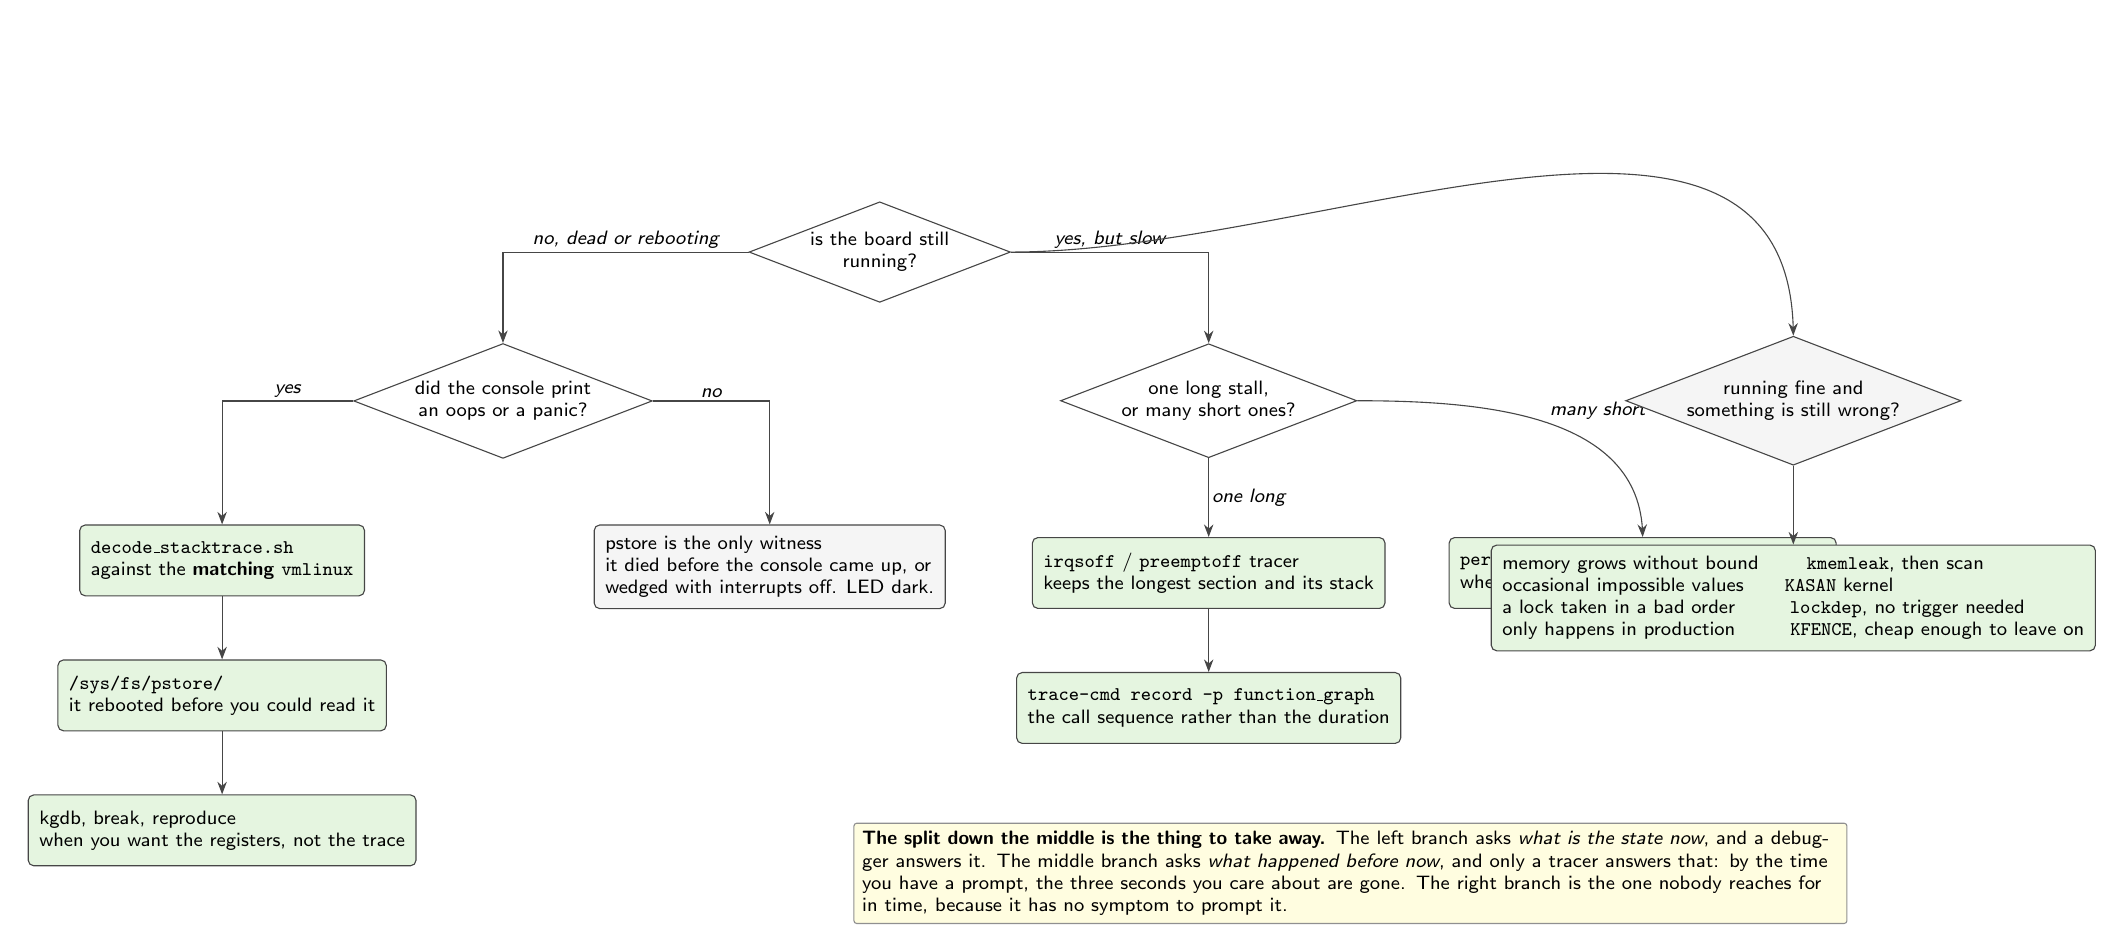
\begin{tikzpicture}[font=\sffamily\small, node distance=8mm]

  \node[qst] (alive) {is the board still\\running?};

  %% ================ branch A: it is not ================
  \node[qst, below left=12mm and 30mm of alive] (oops)
       {did the console print\\an oops or a panic?};
  \draw[trans] (alive) -| node[ans, pos=0.25, above] {no, dead or rebooting} (oops);

  \node[fix, below left=12mm and 8mm of oops] (decode)
       {\texttt{decode\_stacktrace.sh}\\
        \scriptsize against the \textbf{matching} \texttt{vmlinux}};
  \draw[trans] (oops) -| node[ans, pos=0.25, above] {yes} (decode);

  \node[fix, below=8mm of decode] (pstore)
       {\texttt{/sys/fs/pstore/}\\
        \scriptsize it rebooted before you could read it};
  \draw[trans] (decode) -- (pstore);

  \node[fix, below=8mm of pstore] (kgdb1)
       {kgdb, break, reproduce\\
        \scriptsize when you want the registers, not the trace};
  \draw[trans] (pstore) -- (kgdb1);

  \node[fix, below right=12mm and 2mm of oops, fill=quietcol] (silent)
       {pstore is the only witness\\
        \scriptsize it died before the console came up, or\\
        \scriptsize wedged with interrupts off. LED dark.};
  \draw[trans] (oops) -| node[ans, pos=0.25, above] {no} (silent);

  %% ================ branch B: it is running, badly ================
  \node[qst, below right=12mm and 24mm of alive] (slow)
       {one long stall,\\or many short ones?};
  \draw[trans] (alive) -| node[ans, pos=0.25, above] {yes, but slow} (slow);

  \node[fix, below=10mm of slow] (irqsoff)
       {\texttt{irqsoff} / \texttt{preemptoff} tracer\\
        \scriptsize keeps the longest section and its stack};
  \draw[trans] (slow) -- node[ans, right] {one long} (irqsoff);

  \node[fix, right=8mm of irqsoff] (perf)
       {\texttt{perf record -g}\\
        \scriptsize where the time goes, not where it stopped};
  \draw[trans] (slow.east) to[out=0, in=90] node[ans, above right] {many short} (perf.north);

  \node[fix, below=8mm of irqsoff] (fgraph)
       {\texttt{trace-cmd record -p function\_graph}\\
        \scriptsize the call sequence rather than the duration};
  \draw[trans] (irqsoff) -- (fgraph);

  %% ================ branch C: it is fine and wrong ================
  \node[qst, right=34mm of slow, fill=quietcol] (fine)
       {running fine and\\something is still wrong?};
  \draw[trans] (alive.east) to[out=0, in=90] (fine.north);

  \node[fix, below=10mm of fine, align=left] (quiet)
       {memory grows without bound \ \ \ \ \ \ \texttt{kmemleak}, then scan\\
        occasional impossible values \ \ \ \ \ \texttt{KASAN} kernel\\
        a lock taken in a bad order \ \ \ \ \ \ \ \texttt{lockdep}, no trigger needed\\
        only happens in production \ \ \ \ \ \ \ \texttt{KFENCE}, cheap enough to leave on};
  \draw[trans] (fine) -- (quiet);

  %% ---------------- the reading of it ----------------
  \node[umlnote, anchor=north, text width=124mm, align=left]
       at ($(fgraph.south)+(18mm,-10mm)$)
       {\textbf{The split down the middle is the thing to take away.} The
        left branch asks \emph{what is the state now}, and a debugger
        answers it. The middle branch asks \emph{what happened before
        now}, and only a tracer answers that: by the time you have a
        prompt, the three seconds you care about are gone. The right
        branch is the one nobody reaches for in time, because it has no
        symptom to prompt it.};

\end{tikzpicture}
\end{document}
